\chapter{Concepts} \label{chap:concepts}

In this chapter, I will present to the reader a set of concepts that are necessary to fully understand the scope of this document and its implications for the future of scientific research.

\section{Knowledge representation} \label{sec:concepts/knowledge-representation}

As discussed in the introduction, the collective knowledge of mankind is ever increasing, and scientific knowledge is no exception. Measuring this growth is not easy, but the truth of this statement is often illustrated by pictures such as the one in \figref{fig:medline-growth}, which plots the number of articles indexed by MEDLINE through time. This increase seems to be exponential, which can be stated in other words: the amount of knowledge produced depends on the amount of knowledge that exists. The more we know, collectively, as a society, the more we can discover.

With this increase, managing, processing and using the total amount of knowledge becomes more difficult to do. This is where the power of computers can be harnessed to help us in the endeavour of knowledge discovery. The difficulty with this is that knowledge is not directly machine readable. Indeed, established facts have been traditionally published in plain text, which enables humans to understand them; however, natural language processing techniques are not yet fully capable of converting scientific text into \emph{actionable} formats (\eg formats that allow automatic reasoning). Therefore, to enable the application of computerised processing power to knowledge manipulation, it is essential that we find ways to represent knowledge in a machine readable format, which is the subject of Knowledge Representation (KR).

The goal of KR is to find ways to give machines the means to deal with information the same way that humans do, which will ultimately allow them to reason over data and create new knowledge, or at least assist humans to do so. Under this point of view, KR can be (grossly) reduced to two related tasks:
\begin{paralist}
    \item establish the right formats for representing knowledge, and
    \item specify and implement reasoning capabilities that exploit the knowledge thus represented.
\end{paralist}
In this thesis, I will lean on both aspects of KR: first, I will focus on the representation aspect of KR, which provides the information needed to implement similarity measures; second, semantic similarity itself enables reasoning over data (for example, proteins of similar function often have the same sub-cellular localization, and similarity of function can be used to infer this).

However, the subject of KR is vast, with roots in logic, psychology, and even mathematics. I will, therefore, only lightly touch these subject, and always indirectly (as fascinating as it may be, a full treatment of this subject is outside the scope of this document). For example, although I will use the notion of ``Ontologies'' (see next section) as the medium through which knowledge is represented, the full notion of logical formalisms will be mostly absent.

There are two kinds of KR-based reasoning:
\begin{paralist}
    \item deductive reasoning, \ie drawing specific conclusions based on general information (a true fact about animals can be used to deduce a true fact about humans, for example that both are living beings), and
    \item inductive reasoning, \ie drawing general conclusions based on specific data points (a known fact about a large set of mammals can be used to induce that the same fact is true about any mammal, for example after observing that dogs, lions, cats and giraffes have fur, we can induce that all mammals have fur)~\citep[][chap.~1]{Overton2013}.
\end{paralist}
Semantic similarity, being a tool that facilitates automated reasoning, can only be used to produce inductive arguments. However, inductive reasoning is not true reasoning, in the sense that it can reach wrong conclusions (the example above being an illustration of that), but it provides a starting point for further experimentation. For example, semantic similarity can be used to predict a set of probable (but not certain) functions for a given protein, which must then be tested in wet laboratory conditions. Under this context, semantic similarity can be used in techniques such as machine learning to produce new knowledge that is not logically derived from existing one but is instead induced from the starting data.


\section{Ontologies} \label{sec:concepts/ontologies}

The term ``ontology'' was originally used by philosophers, meaning the study of reality, of what exists and how the existing things can be organised and subdivided based on their differences and similarities. The practice of categorising the reality in this manner is in fact an old one, going back to Aristotle (circa 350~BC), who tried to categorise all living things into a hierarchy based on the apparent complexity of their structures and functions, a \emph{scala naturae}, or ``ladder of life'', as it was later called by \citet{Singer1931}.

This term has more recently been borrowed by computer science to mean a particular computational artefact (for example, a computer file, or a database) that contains
\begin{paralist}
    \item a set of concepts belonging to a certain domain of knowledge, and
    \item the ways these concepts relate to each other~\citep{Gruber1993}.
\end{paralist}
One important aspect of computational ontologies is the notion that the ontology actually provides \emph{semantics} (\ie meaning) to the concepts it represents; however, the meaning is not described explicitly, as happens for example in dictionaries and glossaries, but rather \emph{emerges} from the relationships between the concepts and the overall structure of the ontology. Consequently, in a real and useful way, ontologies are machine-readable representations not only of knowledge and facts, but also of the meaning of the concepts pertaining to a given domain of reality, and of the relationships between these concepts.

Within the computer science community, it seems there is no agreed-upon definition of what an ontology is~\citep{Guarino1998}. An oft cited definition is that an ontology is ``an explicit specification of a conceptualization''~\citep{Gruber1993}, but this vague and abstract description makes it difficult to properly visualise the true meaning of the word. In this line of thought, in fact, there are a number of potential information artefacts that can be regarded as ``specifications'' of domains of knowledge, where the main difference between them is their \emph{formality}. \figref{fig:spectrum} presents some possible artefacts that have been at one point in history, regarded as ontologies, arranged by formality levels. The more formal an ontology is, the more precise and expressive is the knowledge it represents.

\begin{figure}
    \centering
    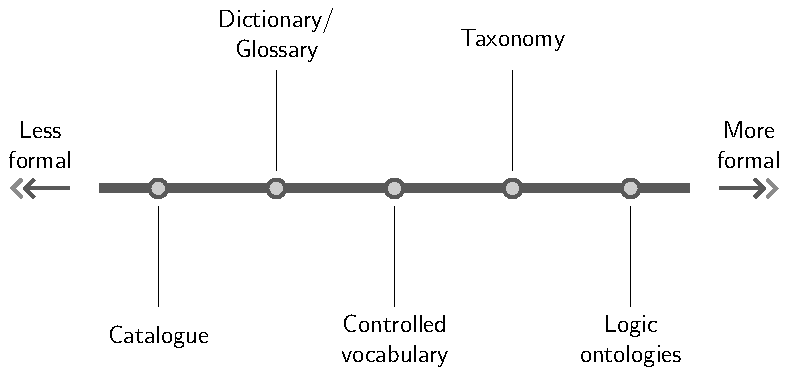
\includegraphics{images/spectrum.pdf}
    \caption[The spectrum of ontology formality]{This picture depicts the possible interpretations of what constitutes an ontology, arranged by formality levels. A \emph{catalogue} is a list of terms, with no definitions or relations between themselves; a \emph{dictionary} provides some textual definitions, as well as, possibly, synonyms; a \emph{controlled vocabulary} defines a standard set of terms to be used in a particular context, along with textual definitions, synonyms, related concepts, \etc.; a \emph{taxonomy} arranges the terms is a hierarchy, without formally defining what it means for a concept to be classified under another concept; and a \emph{logic ontology} provides machine-readable knowledge in a formal and precise way. Many other possible interpretations have been left out of this spectrum. Adapted from~\citep{McGuinness2002}.}
    \label{fig:spectrum}
\end{figure}

This spectrum can be used to distinguish some of the ontologies used by the biomedical informatics community. While the most recent ontologies, including most of the ontologies used in this work, have been developed using formal systems (\ie with the use of formal languages), some have still not been fully formalised. An example is the Medical Subject Headings (\ontology{MeSH}), which is a taxonomy of concepts that are related to one another by means of an underspecified relationship type. For example, \term{Head} is categorised under \term{Body Regions}, and \term{Ear} is categorised under \term{Head}, but while heads are body regions, ears are not heads; they are instead \emph{parts} of the head. This illustrates the informality of \ontology{MeSH}: only one relationship type exists, but it is used to express different notions.

% While most of the semantic similarity algorithms developed so far can be applied to semantic networks in general (to the best of my knowledge, using formal OWL constructions in semantic similarity algorithms has been first attempted in one of my papers~\citep{Ferreira2013}), this thesis will focus mainly on formal ontologies.

Contrast this with the far right end of the spectrum, occupied by fully formal ontologies. In these, complex logic-based assertions can be made about the domain being represented in the ontology. For example, one can express the notions that
\begin{paralist}
    \item \term{Square} and \term{Circle} are disjoint concepts (nothing can exist that is both a square and a circle);
    \item \term{Elephant} is a subclass of \term{Animal} (all elephants are animals); and
    \item a \term{Finger} is \prop{part-of} some \term{Hand}.
\end{paralist}

In order to develop fully formal ontologies, with formal-logic constructions that allow us to assert those types of facts (called \emph{axioms} in KR), several languages have been developed over the years, enabling knowledge engineers to formally represent the concepts of a domain and the relationships between those concepts. The current standard in KR is to use the Web Ontology Language (peculiarly, abbreviated as OWL). This language uses many first-order logic constructions to state facts about the concepts that are represented in the ontologies. OWL ontologies can be saved in files using different but equivalent formats, such as XML, Turtle or JSON. OWL semantics are specified by the World Wide Web Consortium, which defines how each construct should be interpreted and which logical conclusions can be deduced from them~\citep{Motik2012,Motik2012a}.

The most frequent construction in an ontology is the ``class-subclass'' relationship (variously called the \prop{is-a}, ``hypernymy'' or ``subsumption'' relation): \eg the concept \term{Elephant} is a ``hyponym'' of the concept \term{Animal}, since all elephants are animals (likewise, \term{Animal} is a ``hypernym'' of \term{Elephant}). Another common relationship between concepts is ``meronymy'', which is the relationship between the part and the whole, \eg a \term{Finger} is part of some \term{Hand}. A significant portion of the knowledge represented in an ontology can be visualised as a graph, where nodes are concepts and edges are relationships (\eg the class-subclass relationship, or the relationship between part and whole). The hypothetical ontology presented in \figref{fig:anatomy-ontology} shows this parallel between ontologies and graphs. Each of the edges corresponds to one of the axioms of the ontology and, therefore, to an asserted fact. Usually, the class-subclass hierarchy is represented as a tree, while the other relationships are represented as general edges between the nodes.

\begin{sidewaysfigure}
    \centering
    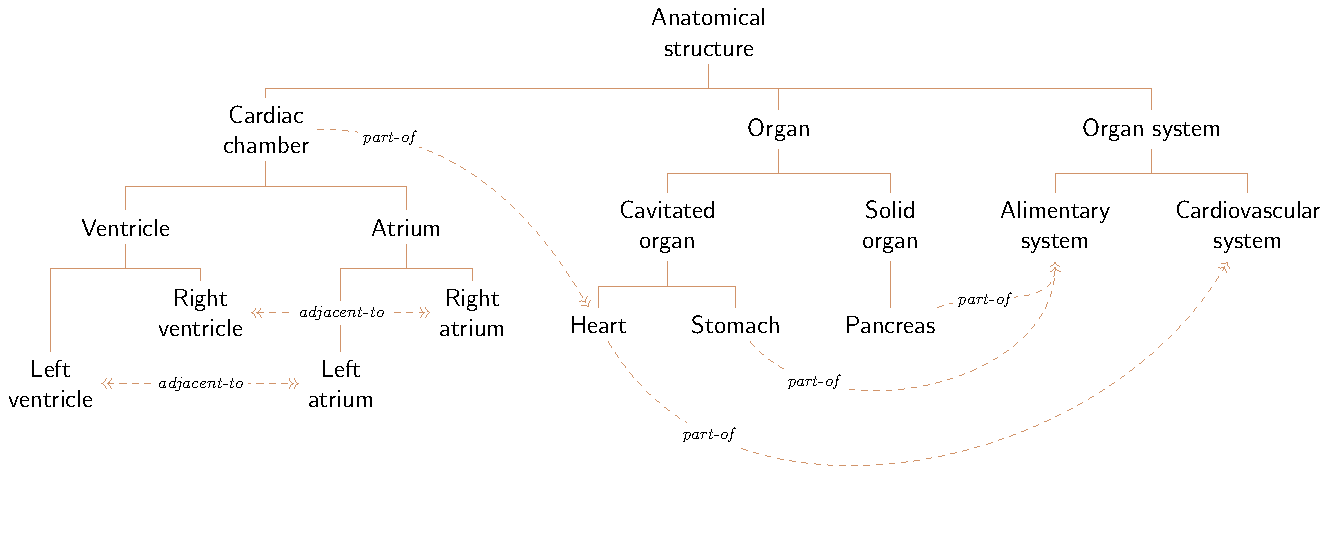
\includegraphics{images/anatomy.pdf}
    \vspace{-\baselineskip}
    \caption[A hypothetical ontology of human anatomical concepts]{This hypothetical ontology contains several concepts related to the domain of human anatomy. It includes concepts that are related to one another by means of the class-subclass relationship (in solid lines) and other types of relationship (in dotted lines, edges labelled with the type of relationship). A note for the reader: this image will be referenced throughout this chapter and the next \mdash take a moment to memorise that this is page number~\pageref{fig:anatomy-ontology}.}
    \label{fig:anatomy-ontology}
\end{sidewaysfigure}

In the biomedical domain, ontologies are often composed of concepts but not of actual instances of these concepts. For example, while the concept for \term{Head} exists in the human anatomy ontology, it being the machine-readable representation of all the human heads, the various instances of this concept (my head, the reader's head, and all human heads that ever existed and will ever exist) are not part of the ontology. In fact, since ontologies are abstractions over reality, they contain only facts that are true for all instances of a particular type. As such, they do not contain instances but instead represent concepts only.

As ontologies are inserted in a computer-science context, developing an ontology is in practice a two-sided task: on the one hand, it requires a logic background, since the formalisms of OWL are founded on first-order logic; on the other hand, it requires a background on the domain being represented in order for the ontology to be as accurate as possible. Beyond these inevitable prerequisites, building an ontology that aspires to be \emph{the} standard representation of a scientific field of research demands a significant commitment to the best practices of ontology development. For example, ontologies should be reusable, the concepts should have textual definitions for the benefit of its human users that are synchronised with the formal definitions (given by the axioms of the ontology that refer to the concepts), and the ontology should be kept updated in light of scientific advances, to guarantee its correctness~\citep{Noy2001}.

Additionally, ontologies should be as interoperable as possible. There is a project within the biomedical informatics community, the OBO Foundry, which specifies a set of principles that are designed to increase the interoperability of the ontologies, such as orthogonality between ontologies and reuse of concepts form one ontology to the next~\citep{Smith2007}. This ensures that each biomedical concept has a single representation and is, therefore, unambiguous.


\section{Web Ontology Language} \label{sec:concepts/owl}

While research on semantic similarity should be agnostic to the languages used to express the ontologies, in practice, the existence of standards and community-driven recommendations means that the majority of ontologies are expressed using the same standards. In fact, the Web Ontology Language~(OWL) is currently the language of choice to represent scientific knowledge, particularly in the biomedical domain. While other languages exist, largely due to historical reasons, they almost always have a translation to OWL.

For example, the OBO Foundry has been active since before OWL had been fully specified, and as such they have developed an ontology language of their own, called OBO (while the name is the same, OBO Foundry and OBO language are distinct concepts). With the standardization of OWL, however, OBO language has been almost completely deprecated: its constructions can be represented in OWL (\ie OBO is, semantically, a subset of OWL), and tools to convert from it to OWL have been developed.

Since my work was based on OWL ontologies, it is important to let the reader know some of the terminology and notation used by this descriptive language.

In general, OWL ontologies are a representation of the concepts that describe the domain of knowledge being encoded in the ontology. The basic object of an OWL ontology is therefore the \emph{class}: the representation of the real-world concept. Another important notion is the \emph{individual}, which is the representation of a real-world object relevant for the domain. For example, a human anatomy ontology would contain the class \term{Heart}, which can be thought of as the set of all the individual ``human hearts'': my heart, the reader's, and all other human hearts that have existed, exist in this moment, and will exist in the future.

OWL ontologies also make use of \emph{properties}, which are the ``verbs'' that represent the relationship between the individuals. For example, ``my heart'' \prop{has-part} ``my left ventricle''. Properties are exclusively asserted between individuals; however, the ontology can describe high-level collections of property assertions that are known to be true. For example, since all human hearts have one left ventricle, a human anatomy ontology contains an \emph{axiom} that represents this fact (see \figref{fig:anatomy-ontology}).

There are several types of axioms that can be asserted in an OWL ontology, which are the constructions of the ontology most closely based on the field of description logic and deductive reasoning. The types of axiom relevant for this work are the following:
\begin{itemize}
    \item The \emph{subclass of} axiom states that all the instances of one class are also instances of the other class: \eg ``$\term{Ventricle} \sqsubseteq \term{Cardiac chamber}$'' means that all ventricles are cardiac chambers.
    \item The \emph{disjointness} axiom between two states that there can never be an object that is simultaneously an instance of the two: \eg ``$\term{Ventricle} \,\sqcap\, \term{Atrium} \sqsubseteq \bot$'' means that there is no object in the real world that is both a ventricle and an atrium.
    \item The \emph{existential quantification} axiom states that instances of a class are related to an instance of another class by a certain property: \eg ``\existential{Heart}{has-part}{Left ventricle}'' means that every heart has a part that is a left ventricle.
\end{itemize}

The logical nature of these axioms are the main reason that ontologies such as \ontology{MeSH} are not on the same formality level than other carefully crafted logical ontologies. For example, a hypothetical axiom ``\existential{Head}{has-part}{Nose}'' (all heads have a nose), together with the fact that \term{Ear} is categorised under \term{Head} in this ontology, would lead to the incorrect inference that every ear has one nose.

While OWL allows the description of individuals, biomedical ontologies are developed and used as reference ontologies for various purposes and, as such, do not define any particular instance of their classes. They only describe the knowledge at the high level of the concepts.

Ontologies in general, and OWL ontologies in particular, make use of what is known as the \emph{open-world assumption}. Informally, this assumption states that what is not asserted does not give any information about what is known \emph{not} to be true. One consequence is that if an ontology does not contain subclasses for a given concept, it cannot be assumed that no such subclasses exist. A highly appropriate quote from Martin Rees~\citep{Oliver1971,Berendzen1973} perfectly encompasses this assumption:
\begin{quote}
    Absence of evidence is not evidence of absence.
\end{quote}
This has significant impact on the rules of inference that are allowed in OWL ontologies, and has consequences to the overall research performed in this area, as we will see later in \chpref{chap:enhancements}.

Being part of an effort to make knowledge more accessible to machines, OWL language uses the idea of \emph{universal identifiers}. The Internationalized Resource Identifier (IRI) are, superficially, similar to URLs. For example, the most abstract concept that can be used in an OWL ontology is \nolinkurl{http://www.w3.org/2002/07/owl\#Thing}, a class that contains all instances. This identifier can be used in any OWL ontology with the meaning defined by the World Wide Web Consortium (W3C). Likewise, any identifier that is a valid IRI can be used by any OWL ontology, and the universal nature of the identifier assures both developer of the ontology and its users that the class represents the concept defined in the ontology where it was originally created.


\section{Semantic web} \label{sec:concepts/semantic-web}

Once knowledge has been made machine-readable by using ontology concepts and entity annotation, it needs to be stored and shared amongst interested parties. This idea of publishing and sharing machine-readable information has been made possible by the semantic web, which prescribes both
\begin{paralist}
    \item a set of standard formats for representing knowledge (of which OWL and IRI are examples); and
    \item a collection of technologies to deal with knowledge (such as reasoning over OWL ontologies).
\end{paralist}
In particular, the semantic web is a vision of information management and sharing that promotes intelligent access to data on the World Wide Web, both by humans and by computers~\citep{Berners-Lee2001,Shadbolt2006}. It is especially useful for handling heterogeneous data, since it was designed with a structured yet flexible operation mode.

The semantic web is build around the idea of expressing information in structured and formal languages, such as the Resource Description Framework (RDF), that allow the expression of precise statements (\eg ``Mary'' \prop{has-father} ``Peter''). At the most basic layer, the semantic web does not define what the property \prop{has-father} means, working instead as a framework for sharing formal statements, which allows users with the necessary knowledge to deal with this information according to their needs. At a higher layer, semantic web \emph{does} use the expressive and logical power of ontologies, enabling data to be effectively searched based on its semantics rather than its syntax. For example, with an ontology that contains the fact that the property \prop{has-father} is the inverse of \prop{father-of}, a user can search in a data repository for the objects~$x$ that satisfy the expression ``Peter'' \prop{father-of}~$x$, and still find the answer ``Mary'' (along with all her siblings, if any exist in the repository): while this exact statement was never introduced in the repository, the inverse statement was, and the relation between the properties \prop{has-father} and \prop{father-of} allows the search engine to correctly \emph{infer} this answer. This illustrates one of the most important characteristics enabled by the semantic web: interoperability of data. On the one hand, information is shared using standard formats; on the other hand, the semantics associated with the information, \ie the meaning and the implications of the data, are formalised based on the precise semantics of the languages used to describe it. This enables data owners to describe their data using as much precision as deemed necessary, while allowing researchers to query the data being as general as they want, while still guaranteeing that the relevant information is retrieved.
\looseness=1

The use of reasoners enables the production of new data, and allows computers to process the structured information based on their actual semantics. An example of semantic web in action can be seen in the work by~\citet{Lopes2012}. These authors have developed a framework capable of integrating structured knowledge from various sources in a single platform, which is enriched with web services that enable \emph{knowledge federation}, \ie the possibility to query data wherever it resides, without the need to add it to a local repository. The formality behind semantic web data suggests that these data can be linked with other information~\citep{Bizer2009, Bizer2009a}, just like documents in the web are linked to each other.

An interesting example of the semantic web in action is the use of linked data to cross information on some epidemiological surges with the characteristics of the locations where these surges started (\eg the socio-economic or environmental conditions). To illustrate, consider a collection of epidemiological surges together with a repository containing characteristics of geographical locations. The search presented in \lstref{lst:sparql} is written in SPARQL, a language that expresses queries over RDF stores (also a standard proposed and promoted under the semantic web movement~\citep{Harris2013}). If presented to the correct data repositories, it would return the characteristics of the places where the ``H1N1 surge of 2009'' started. Then, comparing the returned information with the results for other epidemic surges, it would be possible to detect the characteristics more strongly associated with each one, and to find patterns in the data.

\begin{listing}[t]
\centering
\begin{minted}[gobble=4]{sparql}
    PREFIX epidemic: <http://www.epidemiology.com/data/>
    PREFIX geo: <http://www.geography.com/data/>
    
    SELECT ?characteristic
    WHERE {
        epidemic:H1N1_surge_of_2009 epidemic:surge_started_in ?location .
        ?location geo:has_characteristic ?characteristic .
    }
\end{minted}
\caption[Finding the characteristics of the starting place of an epidemic with SPARQL]{This query retrieves the information we are looking for. Notice that it depends on non-existing repositories (\nolinkurl{http://www.epidemiology.com/data} and \nolinkurl{http://www.geography.com/data}) and, as such, is not functional. Even if these repositories existed, the query would only work if \mintinline{sparql}{geo:has_characteristic} was a superproperty of all the relevant properties.}
\label{lst:sparql}
\end{listing}

Another relevant example of semantic web in action is the Open PHACTS project~\citep{Williams2012}, which provides an integrated and interoperable platform that aims at reducing barriers in pharmacology, specially in the task of drug discovery. The general methodology followed for this endeavour is the adoption of semantic web technologies, such as RDF stores, semantic annotation (see next section), SPARQL queries, \etc.\ which are integrated in the platform, thus building on open standards to ensure wide applicability of the approaches used for integration of data.


\section{Semantic annotation} \label{sec:concepts/semantic-annotation}

Ontologies, standing on their own, define a set of unambiguous, objective and traceable concepts, along with their names, synonyms, and (formal or textual) definitions. However, as knowledge artefacts, ontologies do not \emph{do} anything. Using an analogy, ontologies are to knowledge as the source code of a program is to the program itself. They are specifications packed with a lot of potential, and liberating this potential is possible only with the right set of tools, giving researchers the ability to explore the knowledge they contain. Therefore, it is essential for the advancement of science that the community develops and uses ontologies in a way that can be stacked with current technologies designed for this area. In fact, the knowledge that is stored in an ontology can be quite expressive, depending on its format and how formal its representation is, and can be explored in various ways.

For example, repositories enriched with ontology axioms can be paired with SPARQL to allow intelligent search of data within the repository (see \lstref{lst:sparql}). We will see in \secref{sec:concepts/semantic-similarity} that another such technology is semantic similarity (the primary subject of this document), which calculates similarity between entities based on the knowledge that is associated with them.

Right before discussing semantic similarity, however, it is important to understand \emph{what} is usually compared with this technique. Comparing concepts with concepts is not always useful, and ideally we would like to compare full entities (clinical notes, proteins, disease, \etc.)\ which are usually \emph{annotated} with ontology concepts but are not themselves concepts. For example, a common practice in biology is annotating proteins with their functions. It is almost universally accepted that protein functions are well represented in the Gene Ontology (\ontology{GO}). With this ontology, the information that a gene is responsible for a specific function can be expressed, \eg the protein ``telomerase'' \term{UniProt:Q99973} is annotated in the UniProt database as having the function ``ATP binding'' \term{GO:0005524} and being localised in the ``nuclear matrix'' \term{GO:0016363}). This statement is objective, unambiguous (\ie it does not depend on the researcher that made the statement, nor on any other context), universal, and traceable. Databases like AmiGO~\citep{Carbon2009} are dedicated to managing statements like this.

These annotations can be seen as a semantic description of the protein, since they can be used to, computationally, ascribe to the protein a meaning more complex and informative than simply its sequence. There are automatic tools that reason over \ontology{GO} annotation in order to help interpret the results of experimental procedures. For example, Gene-Set Enrichment Analysis determines, based on the gene expression levels in a wild-type individual \vs those of a mutated individual, which \ontology{GO} molecular functions are most strongly associated with the mutated individuals~\citep{Subramanian2005}. This can help identify, for instance, molecular causes of a disease. Relying on ontology concepts to annotate biomedical entities allows automatic reasoning to be applied directly to them, increasing the amount of automation that can in theory be applied in biomedical research.

In many cases, the annotations of an entity span more than one ontology. In epidemiology, a single dataset may require annotation with diseases, geographical locations, medical procedures, socio-economic conditions, \etc.; kinetic models of chemical reactions use concepts representing chemical compounds and the mathematical equations for the reaction's velocity. Given this multidisciplinarity, it is essential that the standard ontologies used throughout the community can work together, providing users with the confidence that their annotations are interoperable. As discussed previously, this is the case with most ontologies of the biomedical domain. For example, some proteins capture ethanol molecules, a function represented in \ontology{GO} with the concept \term{Ethanol binding}. This concept is related to \term{Ethanol}, itself represented in \ontology{CHEBI}. Such interoperability also has the advantage of minimising the risks of representation duplication (akin to ``code duplication'' in software development).

Finally, semantic annotation is itself a form of knowledge representation. By stating, in a machine-readable format, that some protein performs a certain function in the cell, we are augmenting the amount of knowledge that can be exploited by computational methods.


\section{Semantic similarity} \label{sec:concepts/semantic-similarity}

Now that some preliminary concepts have been introduced, we are finally ready to appreciate the notion of semantic similarity.

Traditionally, computers have been able to compare objects that can be represented either mathematically (\eg vectors) or as strings of characters (\eg gene sequences). However, the algorithms that are used with these structures are context-free: they usually transform the structures without any knowledge of what they represent. With the help of a formal representation of knowledge, computers are given the ability to manipulate concepts that are difficult to represent in a mathematical way.

Knowledge representation (by means of ontologies and semantic annotation) provides the appropriate support for automatic manipulation of information. In this context, semantic similarity is a technique that assigns a numeric value to a pair of concepts or annotated entities based on the similarity of their \emph{meaning}, which is automatically extracted from the ontologies.

For example, there is no directly obvious way to compare two anatomical entities. However, considering the illustration in \figref{fig:anatomy-ontology} (page~\pageref{fig:anatomy-ontology}), it is possible to intuitively understand that, because both a \term{Heart} and a \term{Stomach} are examples of a \term{Cavitated organ}, they are more similar than \term{Heart} and \term{Pancreas}. This intuition can be captured in a formal algorithm: \term{Heart} and \term{Stomach} are both subclasses of the concept \term{Cavitated organ}, while \term{Heart} and \term{Pancreas} are subclasses of the concept \term{Organ}, a less specific concept. The fact that this measure of similarity makes use of the meaning of the concepts, as represented in the ontologies, has impelled the use of the phrase ``semantic similarity'', first used in this context by~\citet{Resnik1995}. Although the meaning of a concept is also non-mathematical, it is possible to use ontologies as proxy for that meaning and KR technologies to manipulate it. For this reason, semantic similarity can also be called ``ontology-based similarity''. For the purpose of this thesis, I define semantic similarity as follows:

\begin{quote}
    A semantic similarity measure is an algorithm that takes as input a pair of ontology concepts (\emph{resp.}~a pair of entities annotated with ontology concepts), and returns a numeric value that reflects how similar the concepts (\emph{resp.}~entities) are; the meaning of the concepts being compared (\emph{resp.} used to annotate the entities) is retrieved from the ontologies where they are defined.
\end{quote}

Semantic similarity has been applied in several areas of research. \citet{Hoehndorf2013} provide a collection of applications that contribute to verifiable scientific advances. Some examples collected by me during my research are:
\begin{itemize}
    \item predicting protein interactions (either physical interaction, as part of the same complex, or less obvious interactions, like being part of the same metabolic pathway)~\citep{Azuaje2004,Guo2006,Wu2006};
    \item predicting sub-cellular location of proteins~\citep{Lei2006};
    \item predicting whether a disease affects a certain body part~\citep{Ferreira2011};
    \item finding protein complexes in protein-protein interaction networks~\citep{Li2010b};
    \item helping the differential diagnosis process by suggesting diseases based on a set of symptoms~\citep{Kohler2009};
    \item predicting chemical properties in small metabolites~\citep{Ferreira2010};
    \item finding new putative uses for drugs that are currently being used (drug repositioning)~\citep{Tan2014};
    \item assisting visualization techniques by finding representative concepts in a large set~\citep{Supek2011};
    \item being part of large information retrieval systems~\citep{Emadzadeh2014};
    \item determining the meaning of ambiguous terms~\citep{McInnes2011,Hu2012,Goeg2014};
    \item improving the classification of clinical texts based on machine-learning~\citep{Garla2012a}; and
    \item assisting text-mining by providing a means to detect similarities in meaning that are not obvious using string-similarity measures~\citep{Spasic2005,Varelas2005} and by disregarding some mined facts if they fail to verify a constraint on semantic similarity~\citep{Lamurias2015}.
\end{itemize}

% In practice, semantic similarity has been primarily calculated for concepts from the same ontology or entities annotated with concepts from the same ontology, never mixing more than one ontology. In \secref{sec:sota/multi}, I will make some references to past literature that uses multiple ontologies, but the truth is that this is a topic that has not yet been properly tackled. In fact, while multiple ontologies have been used to compute semantic similarity, this has never been explored in a \emph{multi-domain} context.

The notion of similarity it tightly coupled with the notion of \emph{relatedness}. From a technical point of view, similarity and relatedness are the same idea: they assign a value to a pair of concepts\slash pair of annotated entities. As such, distinguishing between the two ideas is generally difficult. As a rule of thumb, it has been proposed that similarity is context-independent (it takes into account the concepts being analysed but disregards the application under which they are being compared) and relatedness depends on the goals behind the analysis~\citep{Budanitsky1999}. \citet{Pedersen2007} were amongst the first to make a more formal distinction between these two ideas: similarity is a special case of relatedness that considers only the hypernymy of concepts (the class-subclass hierarchy), while relatedness explores all other kinds of properties in the ontologies.

Take, for instance, the concepts \term{Heart} and \term{Blood}. In the biomedical field, they are closely related, since the function of the former is to pump the latter. In gastronomy, there is little relatedness between the two. Independently of the context, however, a heart is not at all similar to blood: one is an organ, the other a biological fluid (in fact, a liquid tissue).

\begin{figure}
    \centering
    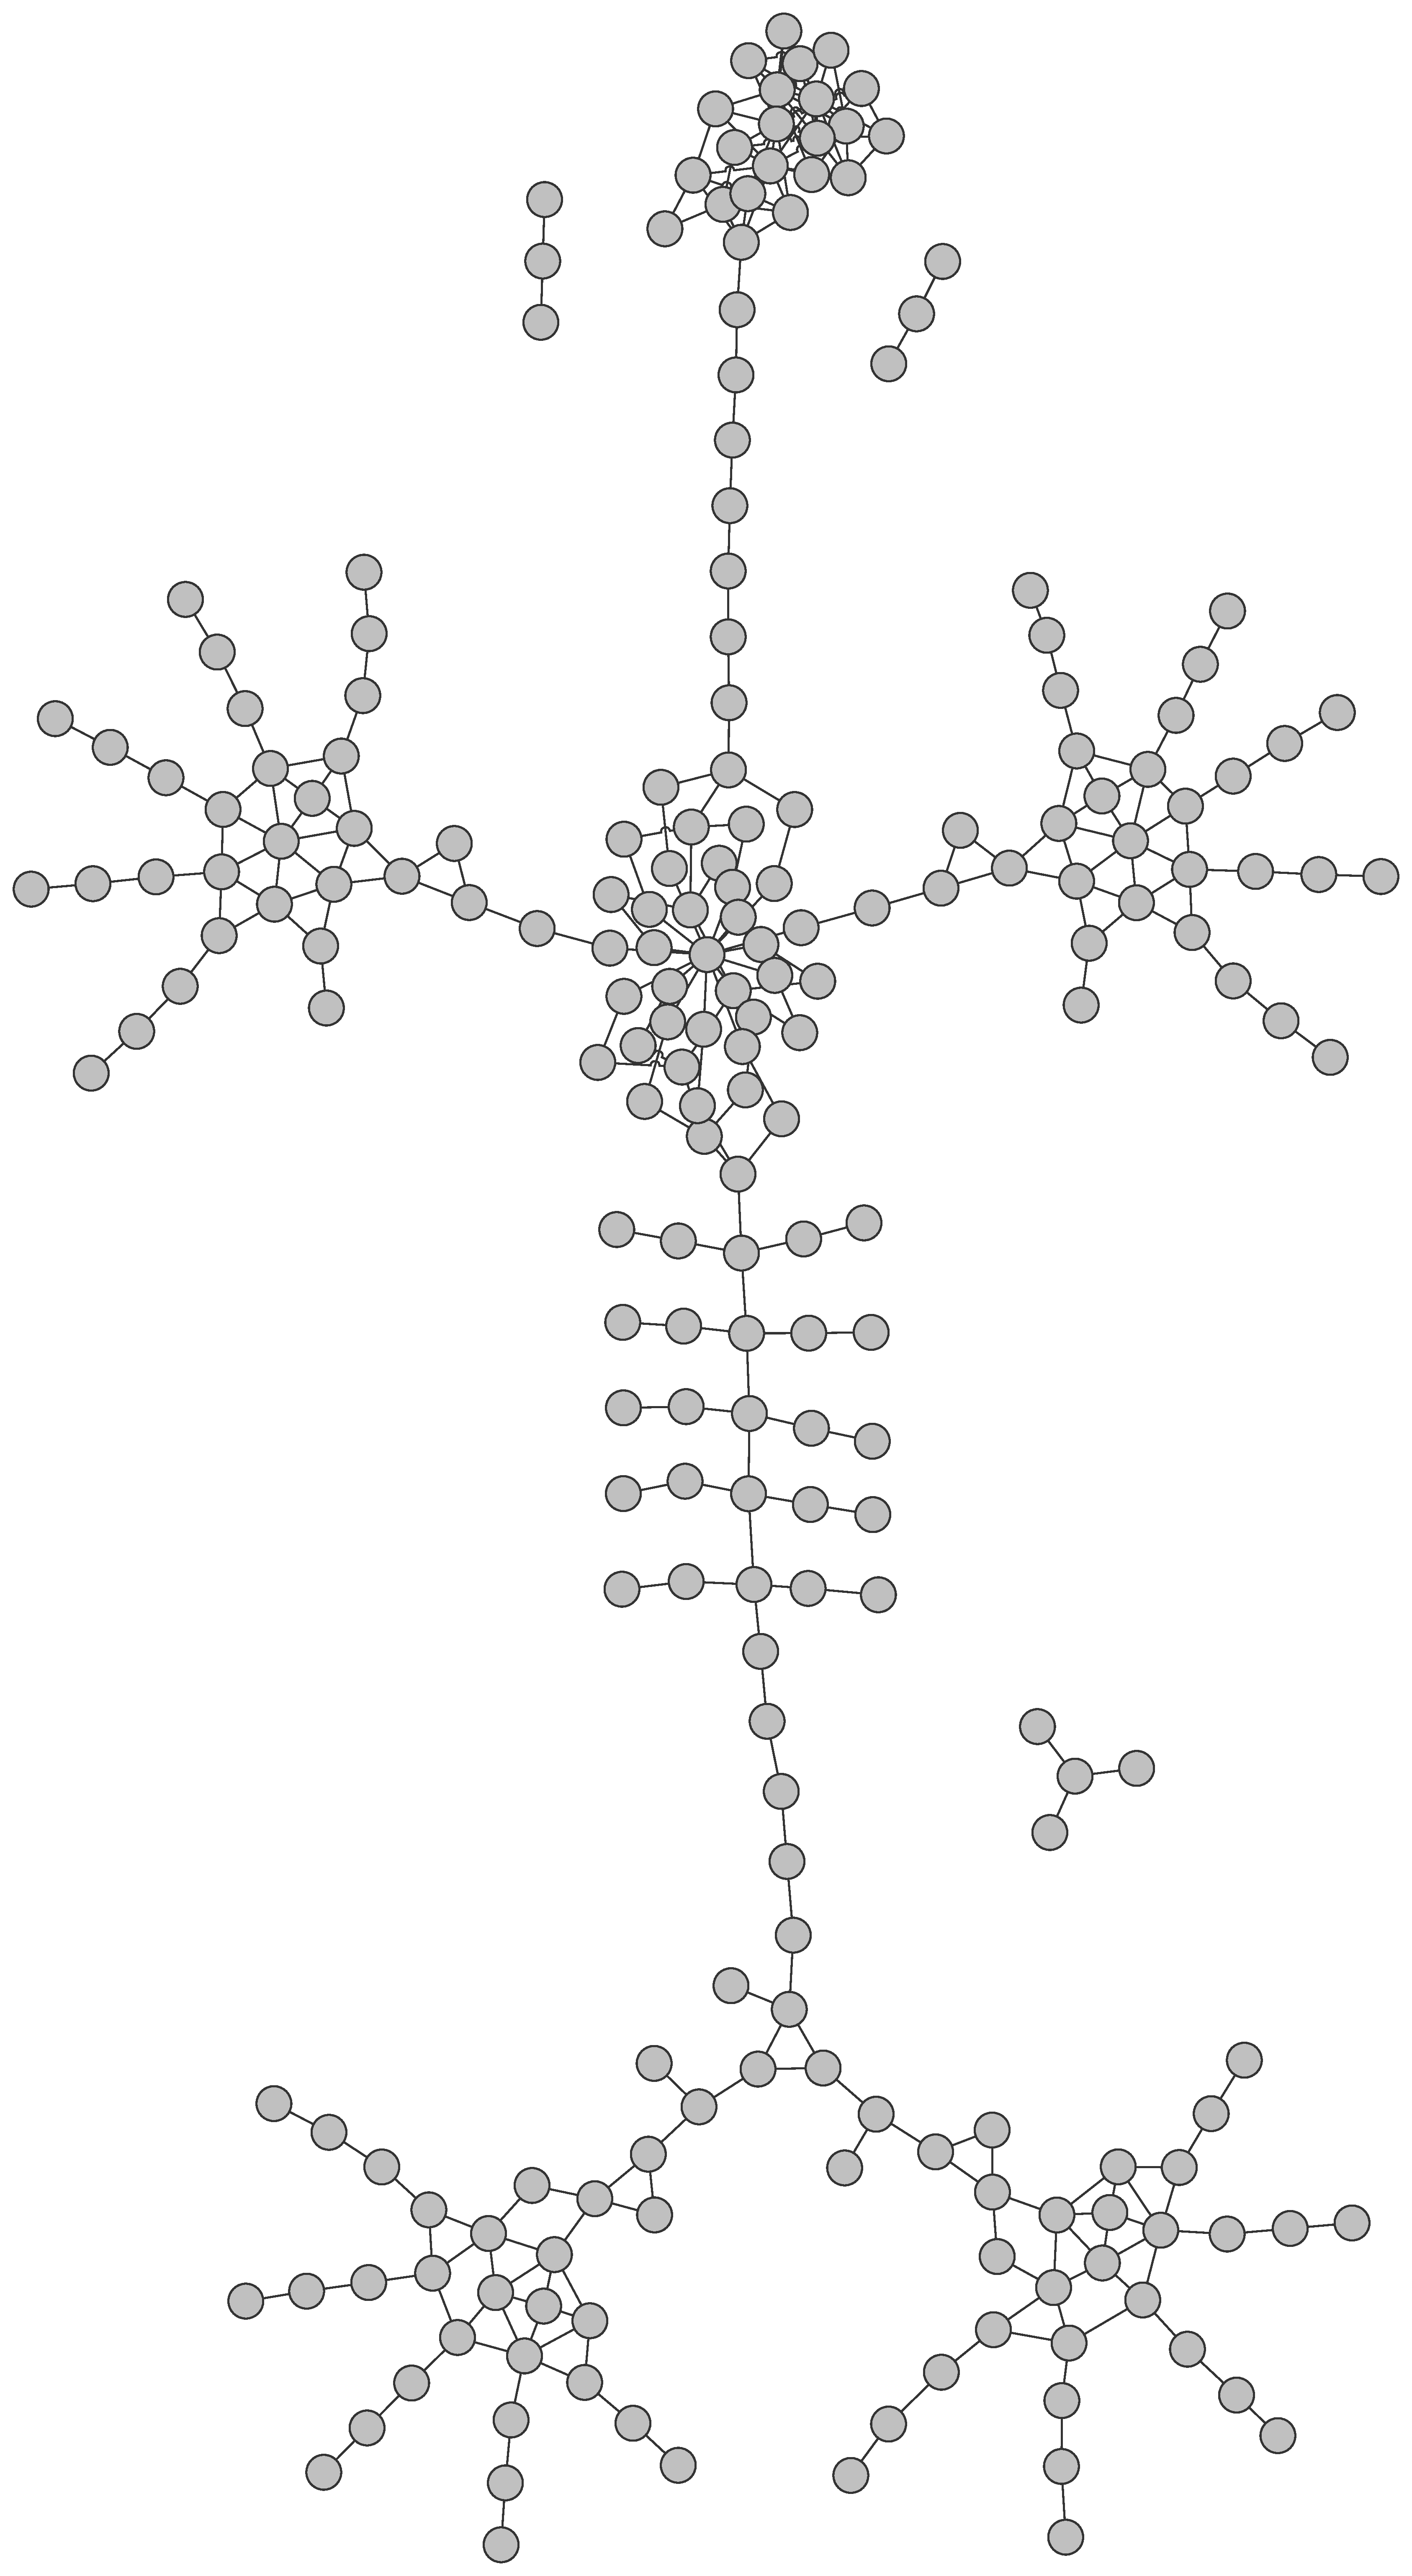
\includegraphics[height=0.7\textheight]{images/skeleton.pdf}
    \caption[Graph describing the \prop{articulates-with} property in \ontology{FMA}]{Each node is a concept from \ontology{FMA} representing a human bone, and each edge represents the fact that the two concepts are related to one another by means of the \prop{articulates-with} property. Features of the human body visible in this picture include: the head, the rib cage, the two hands and their fingers, the ``false ribs'' (which do not articulate with the sternum), the vertebrae, the two feet and their toes, and also the two sets of ear bones, which are disconnected from the rest of the body.}
    \label{fig:skeleton}
\end{figure}

In fact, in some contexts, the use of properties other than the class-subclass relationship can be useful to find patterns in data or to infer new conclusions. Consider the graph drawn in \figref{fig:skeleton}. This figure was obtained by drawing an edge between two anatomical concepts from \ontology{FMA} (the Foundational Model of Anatomy) if the two are related by means of the property \prop{articulates-with}: hence, each node is a bone and the edges show that there is an articulation between the two bones. A graph editor was then used to automatically layout the nodes (I used yEd). Finally, minor manual adjustments were carried out, both to rotate the image and to move the three disconnected subgraphs. Upon closer inspection, it is evident that the graph mirrors a slightly deformed human body, with a head, two hands, a spine, and two feet: the head is tangled because most bones articulate with a large set of other bones, and the rib cage is also tangled because the upper ribs connect both to the spine and the sternum (the two disconnected pieces on the top are the bones of the ear; the third disconnected piece is a bug in the ontology). That this picture is obtained with minimal human intervention and that, even so, it so closely resembles the human body, which is the object being represented in \ontology{FMA}, is extremely provoking evidence that relationships other than hypernymy are vital to properly process scientific knowledge.

In the context of multi-domain similarity, relatedness has, in fact, high utility. Consider now the concepts \term{Otitis} and \term{Ear}, likely to be represented in different ontologies: one for diseases and the other for anatomical entities. Despite being from different ontologies, there is a strong relation between the two, as otitis is an infection of the ear. In the context of diseases, this relationship increases the relatedness between \term{Otitis} and other ear diseases (\eg \term{Hereditary deafness}), which is difficult to capture using similarity alone, since an \term{Otitis} is an inflammatory disease and \term{Hereditary deafness} is a genetic disease. In such a disease hierarchy, it is impossible to obtain an accurate comparison value between the two diseases based on the class-subclass hierarchy only. In fact, we know that \term{Otitis} is an ``\term{Inflammatory disease} that \prop{is-located-in} some \term{Ear}'' and that \term{Hereditary deafness} is a ``\term{Genetic disease} that \prop{manifests-in} some \term{Ear}''. Therefore, exploring the relationships between the concepts other than the class-subclass hierarchy can help increase the accuracy of semantic similarity.

% Incidentally, there are often practical reasons to discourage what is known as the multiple-inheritance pattern in ontology development, \ie the practice of assigning more than one direct superclass to any concept (advantages include an easier development, since errors are easier to debug in this pattern)~\citep{Aranguren2010}. Under this restrain, \term{Otitis} cannot be formally defined as simultaneously an \term{Inflammatory disease} and and \term{Ear disease}.

The concept of distance measures should also be mentioned. Before ontologies were used to compute similarity measures, they were used to compute distances between concepts~\citep{Rada1989}: for a pair of concepts that are close in meaning, similarity values are high and distance values are low. Although there is no unique way to convert a distance into similarity, some formulae have been frequently used. Denoting distance with~$d$ and similarity with~$\sigma$, they are
\begin{itemize}[itemsep=0pt]
    \item $\sigma = 1/d$;
    \item $\sigma = D - d$ where $D$~is the maximum possible distance, and
    \item $\sigma = e^{-\gamma \cdot d}$ for some~$\gamma > 0$.
\end{itemize}
% Distance measures are usually constructed as metrics, satisfying the following three conditions:
% \begin{itemize}[itemsep=0pt]
%     \item identity of indiscernibles:~$\forall x \; d(x, x) = 0$;
%     \item symmetry:~$\forall x,y \; d(x, y) = d(y, x)$; and
%     \item the triangle inequality:~$\forall x,y,z \; d(x, z) \leq d(x, y) + d(y, z)$.
% \end{itemize}
% It has been argued, however, that both symmetry and the triangle inequality can produce unintuitive results when measuring semantic distance between concepts~\citep{Tversky1977,Bowdle1997,Janowicz2007}.




% \section{Information Content} \label{sec:concepts/information-content}

% For a period of time, the notion of an ontology-based semantic similarity measure exploited mainly the distance between two concepts measured in the number of edges between them (see, for an example, the illustration in \figref{fig:distance} for a brief visual summary of that idea). \citet{Resnik1995} introduced the idea of \emph{information content} (IC) to measure how much information is carried out by each concept.

% For example, \term{Animal} can refer to many distinct concepts, and, as such, carries a small amount of information when compared to the concept \term{Dog}, which has a more informative definition. Another way to understand the idea of IC is as a measure of specificity: \term{Dog} is more specific than \term{Animal}. It has been shown that measures that use the notion of IC to weight the concepts of an ontology perform better than those that rely on edges alone~\citep{citation required}. The main reasons for this to happen are that (i) nodes and edges are seldom uniformly distributed throughout the various levels of the class-subclass hierarchy, (ii) edges at the same level do not necessarily correspond to the same semantic distance between concepts and (iii) nodes at the same level do not necessarily have the same specificity~\citep{Pesquita2009}. A simple example shows these faults: the intuitive distance covered by the relationship ``\term{Fungal spore} \prop{is-a} \term{Spore}'' seems to be narrower than the distance in ``\term{Plankton} \prop{is-a} \term{Organism form}'' (examples taken from \ontology{MeSH}).\margin{Maybe use another example from one of the ontologies that will be used in the thesis?}


\section{Multiple-ontology context} \label{sec:concepts/multi-ontology}

As with other emergent fields, the practice of ontology development has been tackled by various people, from hobbyists to philosophers, from scientific research teams that need the power of ontologies for their research, to enterprises that sell their knowledge representation of reality. This can lead to many different ontologies being constructed by different people, with either a different philosophical base or simply a different perspective of reality.

The dissemination of ontology construction and usage places the utility of ontologies in a vantage point, mainly due to two facts:
\begin{paralist}
    \item different interpretations of reality can lead to complementary ontologies, and
    \item a variety of domains of knowledge are getting represented as ontologies, especially by those more competent to do so, \ie people with a background knowledge in these domain.
\end{paralist}

With such a plethora of ontologies available, it is not surprising to notice that many applications are now making use of more than a single ontology. For example, the Epidemic Marketplace~\citep{Lopes2010} uses a number of epidemiology-related ontologies to annotate its resources~\citep{Ferreira2012}, thus connecting a web resource to various concepts from different domains. Another example are models of biological systems, also being annotated with multiple ontologies: with the processes they model, the chemical molecules and cellular components involved in those processes, the physical quantities that they model, \etc.~\citep{Li2010a,Juty2015}. To properly achieve a significant semantic similarity measure between such multidisciplinary entities, it is essential that a multi-domain measure be developed.

\begin{figure}
    \centering
    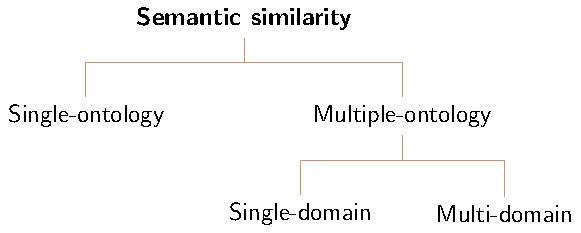
\includegraphics{images/multi-domain-similarity-categories.pdf}
    \caption[Categories of semantic similarity]{Semantic similarity (and relatedness) can be made in a single- or multiple-\emph{ontology} context; but using more than one ontology does not immediately imply a multi-\emph{domain} context, since some ontologies can model the same domains of reality (for example \ontology{MeSH} and \ontology{NCIt} overlap in some of their concepts). As such, multiple-ontology analysis can be further subdivided into single- and multi-domain.}
    \label{fig:multi-domain-similarity}
\end{figure}

Consider the categorization of semantic similarity methods illustrated in \figref{fig:multi-domain-similarity}. Both concepts \term{Heart} and \term{Blood} can be included in an ontology of anatomy and, therefore, their similarity can be computed with a single ontology. However, biomedical ontologies are often incomplete, due to the intrinsic uncertainty associated with the scientific field; they can also contain errors, or can even follow a certain view of reality that is not shared amongst everyone. In each of these cases, a second ontology may be used to offer a complementary view of reality so that incompleteness, errors and subjective interpretations are mitigated. ``Multiple-ontology single-domain'' similarity can be used to handle this situation \citep[\eg][]{Al-Mubaid2009}. In this approach, two or more ontologies representing the same domain are used in a complementary way to improve semantic similarity results.

Multiple-domain similarity represents a step beyond this approach, since it uses multiple ontologies from distinct domains in order to compare concepts in a multidisciplinary context. This is necessary, for example, when performing relatedness analysis, such as when comparing diseases with symptoms, or symptoms with anatomical entities, but also when comparing entities that are annotated with concepts from other domains. For example, the concepts \term{Heart} and \term{Blood}, previously used in the example of single-ontology similarity, can be compared based on their functions, the symptoms they exhibit, or even, if appropriate, their use in gastronomy.


\section{Summary} \label{sec:concepts/summary}

In this chapter, I exposed some of the most important concepts necessary to understand the rest of this document. I started by visiting the notions of knowledge representation and ontologies as computational artefacts, thus laying down a theoretical framework that enables the representation of unstructured information in a way that can be parsed and acted upon by machines. I then mentioned the ideas of semantic web and semantic annotation, which are the response of the scientific community to that theoretical framework: they define the standards that are used to store and share information among the ones representing the knowledge and the ones using that knowledge. At last, I described semantic similarity as one of the techniques that uses information from ontologies, with several possible objectives, and the fact that multi-domain semantic similarity seems to be useful and, yet, underdeveloped.

The next chapter will describe some of the methodologies that have been proposed to calculate semantic similarity, including both historical and state-of-the-art measures.
